\documentclass[12pt, oneside]{book}

\usepackage[a-1b]{pdfx}
\hypersetup{hidelinks, bookmarksnumbered}
\usepackage{tocbibind}

\usepackage[top = 1in, right = 1in, bottom = 1in, left = 1.5in]{geometry}
\pagestyle{plain}
\usepackage[doublespacing]{setspace}

\usepackage[framemethod = tikz, middlelinewidth = 1pt, roundcorner = 3pt]{mdframed}

\usepackage{minted}
\renewcommand{\MintedPygmentize}{./node_modules/.bin/shiki-minted}
\setminted{fontsize = \footnotesize, baselinestretch = 1.2}
\setmintedinline{fontsize = \normalsize}

\usepackage{graphicx, mathpartir}

\usepackage{datetime2} % TODO

\begin{document}

\frontmatter

\begin{center}
\begin{singlespace}
\vspace*{0.5in}

DRAFT: \DTMnow % TODO

\textbf{\uppercase{Yocto-CFA}}

\vspace*{1in}

by\\Leandro Facchinetti

\vspace*{1.5in}

A dissertation submitted to Johns Hopkins University\\in conformity with the requirements for the degree of Doctor of Philosophy

\vspace*{0.5in}

Baltimore, Maryland\\August 2020
\end{singlespace}
\end{center}

\thispagestyle{empty}
\clearpage

% TODO: \chapter{Abstract}

% Not more than 350 words

% \paragraph{Primary Reader and Advisor:}

% Dr.~Scott Fraser Smith.

% \paragraph{Readers:}

% Dr.~Zachary Eli Palmer and Dr.~Matthew Daniel Green.

% TODO: \chapter{Acknowledgements}

% TODO: \chapter{Dedication}

\tableofcontents
% TODO: \listoftables
% TODO: \listoffigures

\mainmatter

% TODO: Introduction
% TODO: Link to GitHub

\chapter{Developing an Analyzer}

% TODO: An overview of the rest of the section

\section{The Analyzed Language: Yocto-JavaScript}
\label{The Analyzed Language: Yocto-JavaScript}

Our first decision when developing an analyzer is which language it should analyze. In this dissertation we are interested in analysis techniques for higher-order functions, a feature which is supported by most languages, including JavaScript, Java, Python, Ruby, and so forth.

From all these options, we would like to choose JavaScript because it is the most popular language among programmers~\cite{stack-overflow-developer-survey, jet-brains-developer-survey}, but JavaScript has many features besides higher-order functions that would complicate our analyzer, so we support only a \emph{subset} of JavaScript features that are related to higher-order functions, resulting in a language that we call \emph{Yocto-JavaScript} ($\mathrm{JavaScript} \times 10^{-24}$). By design, every Yocto-JavaScript program is also a JavaScript program, but the converse does not hold.

\begin{mdframed}[frametitle = {Advanced}]
On the surface the choice of analyzed language is important because it determines how difficult the analyzer is to develop, but the analyzed language may also influence the analyzer's precision and running time. For example, there is an analysis technique called $k$-CFA~\cite{k-cfa} that may be slower when applied to a language with higher-order functions than when applied to a language with objects, because the algorithmic complexity of the former is exponential and of the latter is polynomial~\cite{m-cfa}.
\end{mdframed}

\begin{mdframed}[frametitle = {Technical Terms}]
Yocto-JavaScript is a representation of something called the \emph{$\lambda$-calculus}~\cite[§~6]{understanding-computation}.
\end{mdframed}

\subsection{Values in Yocto-JavaScript}
\label{Values in Yocto-JavaScript}

JavaScript has many kinds of values: strings (for example, \mintinline{js}{"Leandro"}), numbers (for example, \mintinline{js}{29}), arrays (for example, \mintinline{js}{["Leandro", 29]}), objects (for example, \mintinline{js}!{ name: "Leandro", age: 29 }!), and so forth. From all these kinds of values, Yocto-JavaScript supports only one: functions.

An Yocto-JavaScript function is written as \verb!<parameter> => <body>!, for example, \mintinline{js}{x => x}, in which the \verb!<parameter>! is called \mintinline{js}{x} and the \verb!<body>! is a reference to the variable \mintinline{js}{x} (see §~\ref{Operations in Yocto-JavaScript}). An Yocto-JavaScript function must have exactly one parameter. Because an Yocto-JavaScript function is a value, it may be passed as argument in a function call or returned as the result of a function call (see §~\ref{Operations in Yocto-JavaScript}).

\begin{mdframed}[frametitle = {Technical Terms}]
The notation we use for writing functions is something called \emph{arrow function expressions}~\cite{arrow-function-expressions}. The function given as example is called the \emph{identity} function. The ability of acting as values is what characterizes these functions as \emph{higher-order}.
\end{mdframed}

\subsection{Operations in Yocto-JavaScript}
\label{Operations in Yocto-JavaScript}

JavaScript has many operations: strings may have its characters accessed (for example, \mintinline{js}{"Leandro"[2]}, which results in \mintinline{js}{"a"}), numbers may be added together (for example, \mintinline{js}{29 + 1}, which results in \mintinline{js}{30}), and so forth. From all these operations, Yocto-JavaScript supports only two: functions may be called and variables may be referenced.

A function call is written as \verb!<function>(<argument>)!, for example, \mintinline{js}{f(a)}, in which the \verb!<function>! is a hypothetical function \mintinline{js}{f} and the \verb!<argument>! is a hypothetical argument \mintinline{js}{a}. An Yocto-JavaScript function call must have exactly one argument (because an Yocto-JavaScript function must have exactly one parameter; see §~\ref{Values in Yocto-JavaScript}). A variable reference is written as a bare identifier, for example, \mintinline{js}{x}.

The following is a complete Yocto-JavaScript program that exemplifies all the supported operations:

\begin{minted}{js}
(x => x)(y => y)
\end{minted}

This program is a function call in which the \verb!<function>! is \mintinline{js}{x => x} and the \verb!<argument>! is \mintinline{js}{y => y}. When called, an Yocto-JavaScript function returns the result of computing its \verb!<body>! and the \verb!<body>! of \mintinline{js}{x => x} is a reference to the variable \mintinline{js}{x}, so \mintinline{js}{x => x} is a function that returns its argument unchanged and the final result of the example above is \mintinline{js}{y => y}.

In general, all kinds of Yocto-JavaScript expressions (function definitions, function calls, and variable references) may appear in the \verb!<body>! of a function definition, or as the \verb!<function>! or \verb!<argument>! of a call (for example, in the program \mintinline{js}{(f(a))(b)} the function call \mintinline{js}{f(a)} appears as the \verb!<function>! of a call).

We use parentheses to resolve ambiguities on where function definitions start and end, and in which order operations are computed. For example, given hypothetical functions \mintinline{js}{f}, \mintinline{js}{g}, and \mintinline{js}{h}, in \mintinline{js}{(f(g))(h)} the call \mintinline{js}{f(g)} happens first and the result is a function that is called with \mintinline{js}{h}, and in \mintinline{js}{f(g(h))} the call \mintinline{js}{g(h)} happens first and the result is passed as argument to \mintinline{js}{f}.

\begin{mdframed}[frametitle = {Technical Terms}]
The order in which operations are computed is something called their \emph{precedence}, and operations that happen first are said to have \emph{higher precedence}.
\end{mdframed}

\begin{mdframed}[frametitle = {Advanced}]

\subsection{The Computational Power of Yocto-JavaScript}
\label{The Computational Power of Yocto-JavaScript}

Yocto-JavaScript has only a few features, which makes it the ideal language for discussing the analysis of higher-order functions, but is it \emph{too} simple? In other words, in the process of pairing down JavaScript to define Yocto-JavaScript, have we removed features that make the language incapable of some computations? Perhaps surprisingly, the answer is negative: Yocto-JavaScript is equivalent to JavaScript (and Java, Python, Ruby, and so forth) in the sense that, with some effort, any program in any one language may be translated into an equivalent program in any other language~\cite[§~6]{understanding-computation}.

As an example of how to carry out this translation, consider a JavaScript function of two parameters: \mintinline{js}{(x, y) => x}. This function is not supported by Yocto-JavaScript, which supports only functions of one parameter (see §~\ref{Values in Yocto-JavaScript}), but we may encode it as a function that receives the first parameter and returns another function that receives the second parameter: \mintinline{js}{x => (y => x)}. Similarly, we may encode a call with multiple arguments as a sequence of calls that passes one argument at a time, for example, \mintinline{js}{f(a, b)} may be encoded as \mintinline{js}{(f(a))(b)}.

\begin{mdframed}[frametitle = {Technical Terms}]
All the languages we are considering are said to be equivalent in terms of \emph{computational power}: they are all \emph{Turing complete}~\cite[§~7]{understanding-computation}. The translation technique for functions with multiple arguments is called \emph{currying}~\cite[page~163]{understanding-computation}.
\end{mdframed}

For our goal of exploring analysis techniques, we are concerned only with computational power, but it is worth noting that programmers may be more interested in other language properties: Does the language promote writing programs of higher quality? (It most probably does not~\cite{code-quality}.) Does the language improve productivity? Does the language work well for the domain of the problem? (For example, we would probably write an operating system in C and a web application in JavaScript, not the other way around.) Is the language more expressive than others? (Perhaps surprisingly, it is possible to make formal arguments about expressiveness without resorting to personal preference and anecdotal evidence~\cite{expressive-power}.) Despite having the same computational power as other languages, Yocto-JavaScript fares badly in these other aspects: it is remarkably unproductive and inexpressive.

\subsection{A Formal Grammar for Yocto-JavaScript}
\label{A Formal Grammar for Yocto-JavaScript}

The description of Yocto-JavaScript given so far has been informal; the following is a grammar in \emph{Backus–Naur Form}~(BNF)~\cite{bnf}~\cite[§~4.2]{dragon-book} that formalizes it:

\begin{center}
\begin{tabular}{rcll}
$e$ & ::= & $x\texttt{ => }e$ $|$ $e\texttt{(}e\texttt{)}$ $|$ $x$ & Expressions \\
$x$ & ::= & \texttt{<A Valid JavaScript Identifier>} & Variables \\
\end{tabular}
\end{center}

\end{mdframed}

\section{The Analyzer Language: TypeScript}
\label{The Analyzer Language: TypeScript}

After choosing our analyzed language (Yocto-JavaScript; see §~\ref{The Analyzed Language: Yocto-JavaScript}), we must decide in which language to develop the analyzer itself. Our analyzed language is based on JavaScript, but that does not restrict our choice of language in which to develop the analyzer because the analyzer treats the analyzed program as data, so it could be developed in any language: JavaScript, Java, Python, Ruby, and so forth. Still, from all these options, JavaScript does offer some advantages: it is the most popular~\cite{stack-overflow-developer-survey, jet-brains-developer-survey}, and it includes convenient tools to manipulate JavaScript programs (and therefore Yocto-JavaScript programs as well; see §~\ref{Parser} and §~\ref{Step 0: Prettifier}). But JavaScript lacks a way to express the \emph{types} of data structures, functions, and so forth, which we will need (for example, see §~\ref{Data Structures to Represent Yocto-JavaScript Programs}), so we choose to implement our analyzer in a JavaScript extension with support for types called \emph{TypeScript}~\cite{typescript, typescript-deep-dive, understanding-typescript}.

\section{Step 0: Substitution-Based Interpreter}
\label{Step 0: Substitution-Based Interpreter}

Having chosen the analyzed language (Yocto-JavaScript; see §~\ref{The Analyzed Language: Yocto-JavaScript}) and the language in which to develop the analyzer itself (TypeScript; see §~\ref{The Analyzer Language: TypeScript}), we are ready to start the series of Steps in the development of the analyzer. The first Step is an interpreter that executes Yocto-JavaScript programs and produces the same outputs that would be produced by a regular JavaScript interpreter. This is a good starting point for two reasons: first, this interpreter is the basis upon which we will build the analyzer; and second, the outputs of this interpreter are the ground truth against which we will validate the outputs of the analyzer.

\subsection{Architecture}
\label{Architecture}

Our interpreter is defined as a function called \mintinline{ts}{evaluate()}, which receives as parameter an Yocto-JavaScript program represented as a string and returns the result of running it.

\begin{mdframed}[frametitle = {Advanced}]
The \mintinline{ts}{evaluate()} function is named after a native JavaScript function called \mintinline{js}{eval()}, which is similar to \mintinline{ts}{evaluate()} but for JavaScript programs~\cite{eval}.
\end{mdframed}

The following are two examples of how we will be able to use \mintinline{ts}{evaluate()} by the end of this Step (the \mintinline{ts}{>} represents the console):

\begin{minted}{ts}
> evaluate("x => x")
"x => x"
> evaluate("(x => x)(y => y)")
"y => y"
\end{minted}

The implementation of \mintinline{ts}{evaluate()} is separated into three parts called \mintinline{ts}{parse()}, \mintinline{ts}{run()}, and \mintinline{ts}{prettify()}:

\begin{center}
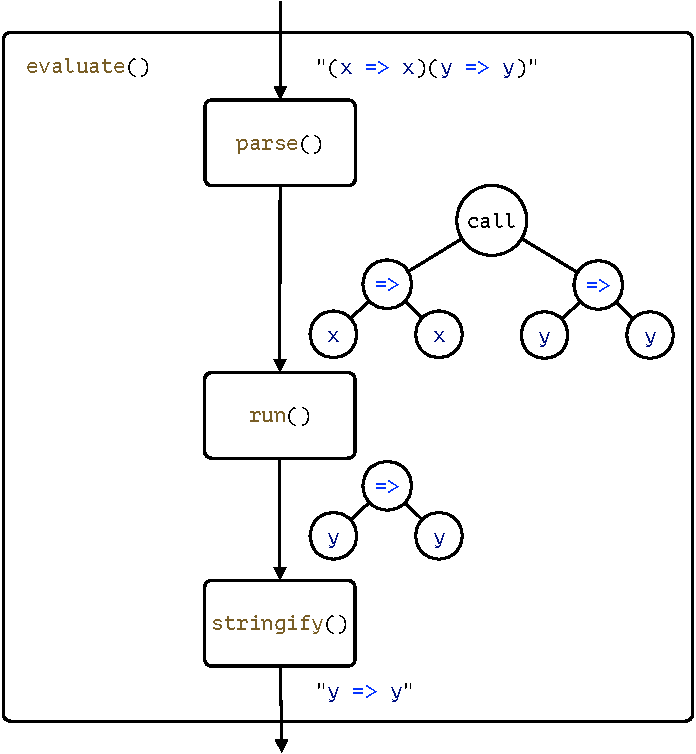
\includegraphics[page = 1]{images.pdf}
\end{center}

\begin{minted}{ts}
export function evaluate(input: string): string {
  return prettify(run(parse(input)));
}
\end{minted}

The \mintinline{ts}{parse()} function prepares the \mintinline{ts}{input} for interpretation, converting it from a string into more convenient data structures (see §~\ref{Data Structures to Represent Yocto-JavaScript Programs}). The \mintinline{ts}{run()} function is responsible for the interpretation itself. The \mintinline{ts}{prettify()} function converts the outputs of \mintinline{ts}{run()} into a human-readable format. In the following sections (§~\ref{Data Structures to Represent Yocto-JavaScript Programs}–§~\ref{An Operational Semantics for the Interpreter}) we address the implementation of \mintinline{ts}{run()}, deferring \mintinline{ts}{parse()} to §~\ref{Parser} and \mintinline{ts}{prettify()} to §~\ref{Step 0: Prettifier}.

In later Steps the implementations of \mintinline{ts}{parse()}, \mintinline{ts}{run()}, and \mintinline{ts}{prettify()} will change, but the architecture and therefore the implementation of \mintinline{ts}{evaluate()} will remain the same.

\subsection{Data Structures to Represent Yocto-JavaScript Programs}
\label{Data Structures to Represent Yocto-JavaScript Programs}

The \mintinline{ts}{evaluate()} function receives an Yocto-JavaScript program represented as a string (see §~\ref{Architecture}), which is convenient for humans to write and read, but inconvenient for \mintinline{ts}{run()} to manipulate directly, because \mintinline{ts}{run()} is concerned with the \emph{structure} of the program instead of the \emph{text}: from \mintinline{ts}{run()}'s perspective it does not matter, for example, whether a function is written as \mintinline{js}{x => x} or as \mintinline{js}{x=>x} (note the difference in spacing). So before \mintinline{ts}{run()} starts interpreting the program, \mintinline{ts}{parse()} transforms it from a string into more convenient data structures (see §~\ref{Parser} for \mintinline{ts}{parse()}'s implementation).

\begin{mdframed}[frametitle = {Technical Terms}]
The process of converting a program represented as a string into more convenient data structures is known as \emph{parsing}, and the data structures are called the \emph{Abstract Syntax Tree}~(AST) of the program~\cite[§~4]{dragon-book}.
\end{mdframed}

The following are two examples of Yocto-JavaScript programs followed by the data structures used to represent them, first in a high-level graphical representation and then in an equivalent low-level textual representation:

\begin{minted}{ts}
> parse("x => x")
\end{minted}
\includegraphics[page = 2]{images.pdf}
\begin{minted}{ts}
{
  "type": "ArrowFunctionExpression",
  "params": [
    {
      "type": "Identifier",
      "name": "x"
    }
  ],
  "body": {
    "type": "Identifier",
    "name": "x"
  }
}
\end{minted}

\begin{minted}{ts}
> parse("(x => x)(y => y)")
\end{minted}
\includegraphics[page = 3]{images.pdf}
\begin{minted}{ts}
{
  "type": "CallExpression",
  "callee": {
    "type": "ArrowFunctionExpression",
    "params": [
      {
        "type": "Identifier",
        "name": "x"
      }
    ],
    "body": {
      "type": "Identifier",
      "name": "x"
    }
  },
  "arguments": [
    {
      "type": "ArrowFunctionExpression",
      "params": [
        {
          "type": "Identifier",
          "name": "y"
        }
      ],
      "body": {
        "type": "Identifier",
        "name": "y"
      }
    }
  ]
}
\end{minted}

We choose to represent Yocto-JavaScript programs with the data structures above because they follow a specification called ESTree~\cite{estree}, and by adhering to this specification we may reuse tools from the JavaScript ecosystem (see §~\ref{Parser} and §~\ref{Step 0: Prettifier}).

In general, the data structures used to represent Yocto-JavaScript programs are of the following types (written as TypeScript types adapted from the ESTree types~\cite{estree-types} to include only the features supported by Yocto-JavaScript):

\begin{minted}{ts}
type Expression = ArrowFunctionExpression | CallExpression | Identifier;

type ArrowFunctionExpression = {
  type: "ArrowFunctionExpression";
  params: [Identifier];
  body: Expression;
};

type CallExpression = {
  type: "CallExpression";
  callee: Expression;
  arguments: [Expression];
};

type Identifier = {
  type: "Identifier";
  name: string;
};
\end{minted}

\begin{mdframed}[frametitle = {Advanced}]
The definitions above correspond to elements of the Yocto-JavaScript grammar (see §~\ref{A Formal Grammar for Yocto-JavaScript}); for example, \mintinline{ts}{Expression} corresponds to $e$.
\end{mdframed}

In later Steps almost everything about the interpreter will change, but the data structures used to represent Yocto-JavaScript programs will remain the same.

\subsection{An Expression That Already Is a Value}
\label{An Expression That Already Is a Value}

\begin{center}
\begin{tabular}{c|c|c}
\textbf{Example Program} & \textbf{Current Output} & \textbf{Desired Output} \\
\mintinline{js}{x => x} & — & \mintinline{js}{x => x} \\
\end{tabular}
\end{center}

We start the definition of \mintinline{ts}{run()} by considering the example above. As mentioned in §~\ref{Data Structures to Represent Yocto-JavaScript Programs}, the \mintinline{ts}{run()} function receives as parameter an Yocto-JavaScript program represented as an \mintinline{ts}{Expression}. The \mintinline{ts}{run()} function is then responsible for interpreting the program and producing a value. In Yocto-JavaScript, the only kind of value is a function (see §~\ref{Values in Yocto-JavaScript}), so we start the implementation of \mintinline{ts}{run()} with the following (we use \mintinline{ts}{throw} as a placeholder for code that has not be written yet to prevent the TypeScript compiler from signaling type errors):

\begin{minted}{ts}
type Value = ArrowFunctionExpression;

function run(expression: Expression): Value {
  throw new Error("NOT IMPLEMENTED YET");
}
\end{minted}

The first thing that \mintinline{ts}{run()} has to do is determine which type of \mintinline{ts}{expression} it is given:

\begin{minted}[highlightlines = {2-9}]{ts}
function run(expression: Expression): Value {
  switch (expression.type) {
    case "ArrowFunctionExpression":
      throw new Error("NOT IMPLEMENTED YET");
    case "CallExpression":
      throw new Error("NOT IMPLEMENTED YET");
    case "Identifier":
      throw new Error("NOT IMPLEMENTED YET");
  }
}
\end{minted}

In our current example, the \mintinline{ts}{expression} already is a \mintinline{ts}{Value}, so it may be returned unchanged:

\begin{minted}[highlightlines = {3}]{ts}
// run()
case "ArrowFunctionExpression":
  return expression;
\end{minted}

\subsection{A Call Involving Immediate Functions}
\label{A Call Involving Immediate Functions}

\begin{center}
\begin{tabular}{c|c|c}
\textbf{Example Program} & \textbf{Current Output} & \textbf{Desired Output} \\
\mintinline{js}{(x => x)(y => y)} & \texttt{NOT IMPLEMENTED YET} & \mintinline{js}{y => y} \\
\end{tabular}
\end{center}

Interpreting function calls is the main responsibility of our interpreter. There are several techniques to do this and in this Step we use one of the simplest: when the interpreter encounters a function call, it substitutes the variable references in the body of the function that is called with the argument that is passed. This is similar to how we reason about functions in mathematics; for example, given the function $f(x) = x + 1$, we calculate $f(29)$ by substituting the references to $x$ in $f$ with the argument $29$: $f(29) = 29 + 1$. The implementation of this substitution technique starts in this section and will only be complete in §~\ref{Substitution in Function Calls}.

\begin{mdframed}[frametitle = {Technical Terms}]
This technique for interpreting function calls is what characterizes our interpreter in this Step as a \emph{substitution-based interpreter}.
\end{mdframed}

In the example we are considering both the function that is called (\mintinline{js}{x => x}) and the argument (\mintinline{js}{y => y}) are immediate functions, as opposed to being the result of other operations, so for now we may limit the interpreter to handle only this case:

\begin{minted}[highlightlines = {3-7}]{ts}
// run()
case "CallExpression":
  if (
    expression.callee.type !== "ArrowFunctionExpression" ||
    expression.arguments[0].type !== "ArrowFunctionExpression"
  )
    throw new Error("NOT IMPLEMENTED YET");
  throw new Error("NOT IMPLEMENTED YET");
\end{minted}

Next, we unpack the called function (using something called \emph{destructuring assignment}~\cite{destructuring-assignment}) and the argument:

\begin{minted}[highlightlines = {8-12}]{ts}
// run()
case "CallExpression":
  if (
    expression.callee.type !== "ArrowFunctionExpression" ||
    expression.arguments[0].type !== "ArrowFunctionExpression"
  )
    throw new Error("NOT IMPLEMENTED YET");
  const {
    params: [parameter],
    body
  } = expression.callee;
  const argument = expression.arguments[0];
  throw new Error("NOT IMPLEMENTED YET");
\end{minted}

Finally, we setup an auxiliary function called \mintinline{ts}{substitute()} that implements the traversal of the \mintinline{ts}{body} looking for references to \mintinline{ts}{parameter} and substituting them:

\begin{center}
\includegraphics[page = 4]{images.pdf}
\end{center}

\begin{minted}[highlightlines = {13-19}]{ts}
// run()
case "CallExpression":
  if (
    expression.callee.type !== "ArrowFunctionExpression" ||
    expression.arguments[0].type !== "ArrowFunctionExpression"
  )
    throw new Error("NOT IMPLEMENTED YET");
  const {
    params: [parameter],
    body
  } = expression.callee;
  const argument = expression.arguments[0];
  const substitutedBody = substitute(body);
  if (substitutedBody.type !== "ArrowFunctionExpression")
    throw new Error("NOT IMPLEMENTED YET");
  return substitutedBody;
  function substitute(expression: Expression): Expression {
    throw new Error("NOT IMPLEMENTED YET");
  }
\end{minted}

Similar to \mintinline{ts}{run()} itself, \mintinline{ts}{substitute()} starts by determining which type of \mintinline{ts}{expression} is passed to it:

\begin{minted}[highlightlines = {2-9}]{ts}
function substitute(expression: Expression): Expression {
  switch (expression.type) {
    case "ArrowFunctionExpression":
      throw new Error("NOT IMPLEMENTED YET");
    case "CallExpression":
      throw new Error("NOT IMPLEMENTED YET");
    case "Identifier":
      throw new Error("NOT IMPLEMENTED YET");
  }
}
\end{minted}

In our current example the \mintinline{ts}{expression} is \mintinline{ts}{x}, an \mintinline{ts}{Identifier}, and it must be substituted with the \mintinline{ts}{argument}:

\begin{center}
\includegraphics[page = 5]{images.pdf}
\end{center}

\begin{minted}[highlightlines = {3}]{ts}
// substitute()
case "Identifier":
  return argument;
\end{minted}

\subsection{Substitution in Function Definitions}
\label{Substitution in Function Definitions}

\begin{center}
\begin{tabular}{c|c|c}
\textbf{Example Program} & \textbf{Current Output} & \textbf{Desired Output} \\
\mintinline{js}{(x => z => x)(y => y)} & \texttt{NOT IMPLEMENTED YET} & \mintinline{js}{z => y => y} \\
\end{tabular}
\end{center}

When \mintinline{ts}{substitute()} (see §~\ref{A Call Involving Immediate Functions}) starts traversing the \mintinline{ts}{body} of the example above, the \mintinline{ts}{expression} is an \mintinline{ts}{ArrowFunctionExpression} (\mintinline{js}{z => x}), and we want substitution to proceed deeper to find and substitute \mintinline{js}{x}, so we call \mintinline{ts}{substitute()} recursively (we use a feature called \emph{spread syntax}~\cite{spread-syntax} to build an \mintinline{ts}{expression} based on the existing one with a new \mintinline{ts}{body}):

\begin{center}
\includegraphics[page = 6]{images.pdf}
\end{center}

\begin{minted}[highlightlines = {3-6}]{ts}
// substitute()
case "ArrowFunctionExpression":
  return {
    ...expression,
    body: substitute(expression.body)
  };
\end{minted}

\subsection{Name Mismatch}

\begin{center}
\begin{tabular}{c|c|c}
\textbf{Example Program} & \textbf{Current Output} & \textbf{Desired Output} \\
\mintinline{js}{(x => z => z)(y => y)} & \mintinline{js}{z => y => y} & \mintinline{js}{z => z} \\
\end{tabular}
\end{center}

The implementation of \mintinline{ts}{substitute()} in the case of \mintinline{ts}{Identifier} introduced in §~\ref{A Call Involving Immediate Functions} \emph{always} substitutes variable references, regardless of whether they refer to the \mintinline{ts}{parameter} of the called function. For example, in the program above \mintinline{ts}{substitute()} is substituting the \mintinline{js}{z} even though the \mintinline{ts}{parameter} is \mintinline{js}{x}. To fix this, we check whether the variable reference matches the \mintinline{ts}{parameter}, and if it does not then we prevent the substitution by retuning the variable reference unchanged:

\begin{minted}[highlightlines = {3}]{ts}
// substitute()
case "Identifier":
  if (expression.name !== parameter.name) return expression;
  return argument;
\end{minted}

\subsection{Name Reuse}

\begin{center}
\begin{tabular}{c|c|c}
\textbf{Example Program} & \textbf{Current Output} & \textbf{Desired Output} \\
\mintinline{js}{(x => x => x)(y => y)} & \mintinline{js}{x => y => y} & \mintinline{js}{x => x} \\
\end{tabular}
\end{center}

In the program above, there are two options for the variable reference \mintinline{js}{x} on the right of the second \mintinline{js}{=>}: it may refer to the first (outer) \mintinline{js}{x} on the left of the first \mintinline{js}{=>}, in which case the output of the program would be \mintinline{js}{x => y => y}; or it may refer to the second (inner) \mintinline{js}{x} on the left of the second \mintinline{js}{=>}, in which case the output of the program would be \mintinline{js}{x => x}:

\begin{center}
\includegraphics[page = 7]{images.pdf}
\end{center}

Currently \mintinline{ts}{substitute()} is implementing Option~1, but this leads to a serious issue: we are not able to reason about the inner function \mintinline{js}{x => x} independently; we must know where it appears and whether a variable called \mintinline{js}{x} is already defined there.

\begin{mdframed}[frametitle = {Technical Terms}]
We say that the problem with Option~1 is that it defeats something called \emph{local reasoning}. We say that Option~2 exhibits a behavior called \emph{shadowing}, and that the outer \mintinline{js}{x} is \emph{shadowed} by the inner \mintinline{js}{x}, because there is no way to refer to the outer \mintinline{js}{x} from the body of the inner function.
\end{mdframed}

We avoid this issue by modifying \mintinline{ts}{substitute()} to implement Option~2, which is also the choice of JavaScript and every other popular programming language. We change \mintinline{ts}{substitute()}'s behavior when encountering a function definition so that if the parameter of the function definition matches the parameter that \mintinline{ts}{subsitute()} is looking for, then \mintinline{ts}{subsitute()} returns the function unchanged, preventing further substitution (note that there is no recursive call to \mintinline{ts}{substitute()} in this case):

\begin{minted}[highlightlines = {3}]{ts}
// substitute()
case "ArrowFunctionExpression":
  if (expression.params[0].name === parameter.name) return expression;
  return {
    ...expression,
    body: substitute(expression.body)
  };
\end{minted}

\subsection{Substitution in Function Calls}
\label{Substitution in Function Calls}

\begin{center}
\begin{tabular}{c|c|c}
\textbf{Example Program} & \textbf{Current Output} & \textbf{Desired Output} \\
\mintinline{js}{(x => z => x(x))(y => y)} & \texttt{NOT IMPLEMENTED YET} & \mintinline{js}{z => (y => y)(y => y)} \\
\end{tabular}
\end{center}

This case is similar to §~\ref{Substitution in Function Definitions}: all \mintinline{ts}{substitute()} has to do is continue traversing the function call recursively:

\begin{minted}[highlightlines = {3-7}]{ts}
// substitute()
case "CallExpression":
  return {
    ...expression,
    callee: substitute(expression.callee),
    arguments: [substitute(expression.arguments[0])]
  };
\end{minted}

\subsection{An Argument That Is Not Immediate}
\label{An Argument That Is Not Immediate}

\begin{center}
\begin{tabular}{c|c|c}
\textbf{Example Program} & \textbf{Current Output} & \textbf{Desired Output} \\
\mintinline{js}{(x => z => x)((a => a)(y => y))} & \texttt{NOT IMPLEMENTED YET} & \mintinline{js}{z => y => y} \\
\end{tabular}
\end{center}

In all example programs we considered so far the argument to a function call was an immediate function definition, but in general arguments may be the result of function calls themselves. We fix this by calling \mintinline{ts}{run()} recursively on the argument (we also remove the check that the argument is an immediate function definition; if it is, then the recursive call to \mintinline{ts}{run()} returns the immediate function unchanged; see §~\ref{An Expression That Already Is a Value}):

\begin{minted}[highlightlines = {3-4, 9}]{ts}
// run()
case "CallExpression":
  if (expression.callee.type !== "ArrowFunctionExpression")
    throw new Error("NOT IMPLEMENTED YET");
  const {
    params: [parameter],
    body
  } = expression.callee;
  const argument = run(expression.arguments[0]);
  const substitutedBody = substitute(body);
  if (substitutedBody.type !== "ArrowFunctionExpression")
    throw new Error("NOT IMPLEMENTED YET");
  return substitutedBody;
  function substitute(expression: Expression): Expression {
    // ...
  }
\end{minted}

\begin{mdframed}[frametitle = {Technical Terms}]
This technique of calling \mintinline{ts}{run()} recursively to produce an immediate function for the argument characterizes the interpreter as \emph{big-step}.
\end{mdframed}

\begin{mdframed}[frametitle = {Advanced}]
The notion that the argument is interpreted to produce a value as soon as the function call is encountered characterizes Yocto-JavaScript as a \emph{call-by-value} language~\cite{call-by-name-call-by-value-and-the-lambda-calculus}. JavaScript itself and most other popular programming languages are call-by-value as well, the most notable exception being Haskell, which is a \emph{call-by-need} language. In a call-by-need language the argument is only interpreted if it is \emph{needed}, for example, if it is used in the function position of another call (see §~\ref{A Function That Is Not Immediate}), or if it is the result of the program (see §~\ref{Continuing to Run After a Function Call}). In a call-by-need language the result of the program above would be \mintinline{js}{z => ((a => a)(y => y))}. There is yet another policy for when to interpret arguments called \emph{call-by-name}: the difference between call-by-name and call-by-need is that in a call-by-name language the an argument may be computed multiple times if it is used multiple times, but in a call-by-need language an argument is guaranteed to be computed at most once.
\end{mdframed}

\subsection{A Function That Is Not Immediate}
\label{A Function That Is Not Immediate}

\begin{center}
\begin{tabular}{c|c|c}
\textbf{Example Program} & \textbf{Current Output} & \textbf{Desired Output} \\
\mintinline{js}{((z => z)(x => x))(y => y)} & \texttt{NOT IMPLEMENTED YET} & \mintinline{js}{y => y} \\
\end{tabular}
\end{center}

This is the dual of §~\ref{An Argument That Is Not Immediate} for the called function, and the solution is the same: to call \mintinline{ts}{run()} recursively (we also remove the check of whether the function is immediate):

\begin{minted}[highlightlines = {6}]{ts}
// run()
case "CallExpression":
  const {
    params: [parameter],
    body
  } = run(expression.callee);
  const argument = run(expression.arguments[0]);
  const substitutedBody = substitute(body);
  if (substitutedBody.type !== "ArrowFunctionExpression")
    throw new Error("NOT IMPLEMENTED YET");
  return substitutedBody;
  function substitute(expression: Expression): Expression {
    // ...
  }
\end{minted}

\subsection{Continuing to Run After a Function Call}
\label{Continuing to Run After a Function Call}

\begin{center}
\begin{tabular}{c|c|c}
\textbf{Example Program} & \textbf{Current Output} & \textbf{Desired Output} \\
\mintinline{js}{(x => (z => z)(x))(y => y)} & \texttt{NOT IMPLEMENTED YET} & \mintinline{js}{y => y} \\
\end{tabular}
\end{center}

This is similar to §~\ref{An Argument That Is Not Immediate} and §~\ref{A Function That Is Not Immediate}: the result of substitution may be not an immediate function but another call, and more work may be necessary to interpret it. We solve this with yet another recursive call to \mintinline{ts}{evaluate()} (we also remove yet another check and inline the \mintinline{ts}{substitutedBody} variable):

\begin{minted}[highlightlines = {8}]{ts}
// run()
case "CallExpression":
  const {
    params: [parameter],
    body
  } = run(expression.callee);
  const argument = run(expression.arguments[0]);
  return run(substitute(body));
  function substitute(expression: Expression): Expression {
    // ...
  }
\end{minted}

\subsection{A Reference to an Undefined Variable}

\begin{center}
\begin{tabular}{c|c|c}
\textbf{Example Program} & \textbf{Current Output} & \textbf{Desired Output} \\
\mintinline{js}{(x => y)(y => y)} & \texttt{NOT IMPLEMENTED YET} & \texttt{Reference to undefined variable: y} \\
\end{tabular}
\end{center}

The only case in which \mintinline{ts}{run()} may encounter a variable reference directly is if the referenced variable is undefined, otherwise \mintinline{ts}{substitute()} would have already substituted it (see §~\ref{A Call Involving Immediate Functions}–§~\ref{Continuing to Run After a Function Call}). In this case, we throw an exception:

\begin{minted}[highlightlines = {3}]{ts}
// run()
case "Identifier":
  throw new Error(`Reference to undefined variable: ${expression.name}`);
\end{minted}

Note that if the reference to an undefined variable occurs in the body of a function that is not called, then we do not reach the case addressed in this section and an exception is not thrown. For example, the result of running the program \mintinline{js}{x => y} is \mintinline{js}{x => y}, not an exception. This is consistent with JavaScript's behavior.

\subsection{The Entire Runner}
\label{The Entire Runner}

The implementation of the \mintinline{ts}{run()} function is complete:

\begin{minted}[linenos]{ts}
type Value = ArrowFunctionExpression;

function run(expression: Expression): Value {
  switch (expression.type) {
    case "ArrowFunctionExpression":
      return expression;
    case "CallExpression":
      const {
        params: [parameter],
        body
      } = run(expression.callee);
      const argument = run(expression.arguments[0]);
      return run(substitute(body));
      function substitute(expression: Expression): Expression {
        switch (expression.type) {
          case "ArrowFunctionExpression":
            if (expression.params[0].name === parameter.name) return expression;
            return {
              ...expression,
              body: substitute(expression.body)
            };
          case "CallExpression":
            return {
              ...expression,
              callee: substitute(expression.callee),
              arguments: [substitute(expression.arguments[0])]
            };
          case "Identifier":
            if (expression.name !== parameter.name) return expression;
            return argument;
        }
      }
    case "Identifier":
      throw new Error(`Reference to undefined variable: ${expression.name}`);
  }
}
\end{minted}

\subsection{A Program That Does Not Terminate}

\begin{center}
\begin{tabular}{c|c|c}
\textbf{Example Program} & \textbf{Current Output} & \textbf{Desired Output} \\
\mintinline{js}{(f => f(f))(f => f(f))} & \texttt{DOES NOT TERMINATE} & \texttt{DOES NOT TERMINATE} \\
\end{tabular}
\end{center}

Yocto-JavaScript may express any program that a computer may run (see §~\ref{The Computational Power of Yocto-JavaScript}), including some programs that do not terminate. For example, consider the program above: on the first call to \mintinline{js}{run()} both the called function and the argument are immediate functions (they are both \mintinline{js}{f => f(f)}), so the first two recursive calls to \mintinline{ts}{run()} (see §~\ref{The Entire Runner}, lines 11 and 12) return the functions unchanged. At this point, the \mintinline{ts}{parameter} is \mintinline{ts}{f}, the \mintinline{ts}{body} is \mintinline{js}{f(f)}, and the \mintinline{ts}{argument} is \mintinline{js}{f => f(f)}. The result of the call to \mintinline{ts}{substitute()} (see §~\ref{The Entire Runner}, line 13) is \mintinline{js}{(f => f(f))(f => f(f))}, which is the same as the initial program, so the recursive call to \mintinline{ts}{run()} (see §~\ref{The Entire Runner}, line 13) leads to an infinite loop.

This is what we expect from an interpreter, but not from an analyzer, which must always terminate. In the next Steps we will transform this interpreter to turn it into an analyzer, and one of the main issues we will address is termination.

\begin{mdframed}[frametitle = {Advanced}]
\subsection{An Operational Semantics for the Interpreter}
\label{An Operational Semantics for the Interpreter}

What we accomplished so far in this section is more than defining an interpreter for Yocto-JavaScript, we also defined formally the \emph{meaning} of Yocto-JavaScript programs: an Yocto-JavaScript program means what the interpreter produces for it. The definition of the meaning of programs in a language is something called the \emph{semantics} of the language, and there are several techniques to specify semantics; the one we are using so far is known as a \emph{definitional interpreter}~\cite{definitional-interpreters}.

A definitional interpreter has some advantages over other techniques for specifying semantics: it is easier to understand for most programmers, and it is executable. But a definitional interpreter also has one disadvantage: to understand the meaning of an Yocto-JavaScript program we have to understand an interpreter written in TypeScript. To address this, other techniques for defining semantics do not depend on other programming languages, and in this section we introduce one of them: \emph{operational semantics}~\cite{operational-semantics, semantics-engineering, pl}.

First, we extend the grammar from §~\ref{A Formal Grammar for Yocto-JavaScript} with the notion of values that is equivalent to the type \mintinline{ts}{Value} (see §~\ref{The Entire Runner}, line 1):

\begin{center}
\begin{tabular}{rcll}
$v$ & ::= & $x\texttt{ => }e$ & Values \\
\end{tabular}
\end{center}

Next, we provide \emph{inference rules} that are equivalent to the behavior of \mintinline{ts}{run()} (see §~\ref{The Entire Runner}, lines 3–36):

\begin{mathpar}
\inferrule [Value]
{ }
{v \Rightarrow v}

\inferrule [Function Call]
{
e_{f} \Rightarrow x_{p}\texttt{ => }e_{b} \\
e_{a} \Rightarrow v_{a} \\
e_{b}[x_{p} \backslash v_{a}] \Rightarrow v \\
}
{e_{f}\texttt{(}e_{a}\texttt{)} \Rightarrow v}
\end{mathpar}

Finally, we provide a \emph{metafunction} that is equivalent to the behavior of \mintinline{ts}{substitute()} (see §~\ref{The Entire Runner}, lines 14–32):

\begin{center}
\begin{tabular}{rcll}
$(x\texttt{ => }e)[x_{p} \backslash v_{a}]$ & = & $x\texttt{ => }(e[x_{p} \backslash v_{a}])$ & if $x \neq x_{p}$ \\
$(x_{p}\texttt{ => }e)[x_{p} \backslash v_{a}]$ & = & $x_{p}\texttt{ => }e$ & \\
$(e_{f}\texttt{(}e_{a}\texttt{)})[x_{p} \backslash v_{a}]$ & = & $(e_{f}[x_{p} \backslash v_{a}])\texttt{(}(e_{a}[x_{p} \backslash v_{a}])\texttt{)}$ & \\
$x[x_{p} \backslash v_{a}]$ & = & $x$ & if $x \neq x_{p}$ \\
$x_{p}[x_{p} \backslash v_{a}]$ & = & $v_{a}$ & \\
\end{tabular}
\end{center}
\end{mdframed}

\subsection{Parser}
\label{Parser}

The parser is responsible for converting an Yocto-JavaScript program written as a string into data structures that are more convenient for the runner to manipulate (see §~\ref{Architecture} and §~\ref{Data Structures to Represent Yocto-JavaScript Programs} for the reasoning and the definition of the data structures). We choose to represent Yocto-JavaScript programs with data structures that are compatible with a specification for representing JavaScript programs called ESTree~\cite{estree, estree-types} because it allows us to reuse tools from the JavaScript ecosystem, including a parser called Esprima~\cite{esprima}, and the Esprima Interactive Online Demonstration~\cite{esprima-demonstration}, which shows the data structures used to represent a given program.

Our strategy to implement the Yocto-JavaScript parser is to delegate most of the work to Esprima and check that the program is using only features supported by Yocto-JavaScript. The following is the full implementation of the parser:

\begin{minted}[linenos]{ts}
function parse(input: string): Expression {
  const program = parseScript(input, {}, checkFeatures);
  const expression = (program as any).body[0].expression as Expression;
  return expression;
  function checkFeatures(node: Node): void {
    switch (node.type) {
      case "Program":
        if (node.body.length !== 1)
          throw new Error(
            "Unsupported Yocto-JavaScript feature: Program with multiple statements"
          );
        break;
      case "ExpressionStatement":
        break;
      case "ArrowFunctionExpression":
        break;
      case "CallExpression":
        if (node.arguments.length !== 1)
          throw new Error(
            "Unsupported Yocto-JavaScript feature: CallExpression with multiple arguments"
          );
        break;
      case "Identifier":
        break;
      default:
        throw new Error(`Unsupported Yocto-JavaScript feature: ${node.type}`);
    }
  }
}
\end{minted}

\begin{description}
\item [Line 1:]

The parser is defined as a function called \mintinline{ts}{parse()}, which receives the program \mintinline{ts}{input} represented as a \mintinline{ts}{string} and returns an \mintinline{ts}{Expression} (see §~\ref{Data Structures to Represent Yocto-JavaScript Programs}).

\item [Line 2:]

Call the Esprima function \mintinline{ts}{parseScript()}, which parses the \mintinline{ts}{input} as if it were a JavaScript program and produces a data structure following the ESTree specification. The \mintinline{ts}{parseScript()} function also detects syntax errors, for example, in the program \mintinline{js}{x =>}, which is missing the function body. We pass as argument to \mintinline{ts}{parseScript()} a function called \mintinline{ts}{checkFeatures()} which is called with every fragment of data structure that represents a part of the program. The purpose of \mintinline{ts}{checkFeatures()} is to check that the program uses only the features that are supported by Yocto-JavaScript.

\item [Line 3:]

Extract the single \mintinline{ts}{Expression} from within the \mintinline{ts}{Program} returned by \mintinline{ts}{parseScript()}. The \mintinline{ts}{as <something>} forms sidestep the TypeScript type checker and assert that the \mintinline{ts}{expression} is of the correct type. This is safe to do because of \mintinline{ts}{checkFeatures()}.

\item [Line 5:]

The \mintinline{ts}{checkFeatures()} function, which is passed to Esprima's \mintinline{ts}{parseScript()} is called with every fragment of data structure used to represent the program. These fragments are called \emph{nodes}, because the data structure as a whole forms a \emph{tree}, also known as the \emph{Abstract Syntax Tree}~(AST) of the program (see §~\ref{Data Structures to Represent Yocto-JavaScript Programs}). The \mintinline{ts}{checkFeatures()} does not return anything (\mintinline{ts}{void}); its purpose is only to throw an exception in case the program uses a feature that is not supported by Yocto-JavaScript.

\item [Lines 6, 7, 13, 15, 17, 23, 25:]

Similar to \mintinline{ts}{run()} and \mintinline{ts}{substitute()} (see §~\ref{The Entire Runner}), \mintinline{ts}{checkFeatures()} starts by determining which type of \mintinline{ts}{Node} it is given.

\item [Lines 8–11:]

Check that the \mintinline{ts}{Program} contains a single statement. This prevents programs such as \mintinline{js}{x => x; y => y}.

\item [Lines 13, 15:]

\mintinline{ts}{ExpressionStatement}s and \mintinline{ts}{ArrowFunctionExpression}s are supported in Yocto-JavaScript unconditionally. We could check that the \mintinline{ts}{ArrowFunctionExpression} includes only one parameter and that this parameter is a variable (as opposed to being a pattern such as \mintinline{js}{[x, y]}, for example), but this would be redundant because Esprima already calls \mintinline{ts}{checkFeatures()} with other unsupported \mintinline{ts}{node}s that subsume these cases. For example, in the program \mintinline{js}{(x, y) => x}, which is a function of multiple parameters, Esprima calls \mintinline{ts}{checkFeatures()} with a \mintinline{ts}{node} of type \mintinline{ts}{SequenceExpression}. Similarly, in the program \mintinline{js}{([x, y]) => x}, which is a function in which the parameter is a pattern, Esprima calls \mintinline{ts}{checkFeatures()} with a \mintinline{ts}{node} of type \mintinline{ts}{ArrayExpression}.

\item [Lines 18–21:]

Check that the \mintinline{ts}{CallExpression} contains a single argument. This prevents programs such as \mintinline{js}{f(a, b)}.

\item [Line 23:]

\mintinline{ts}{Identifier}s are supported in Yocto-JavaScript unconditionally. Note that an \mintinline{ts}{Identifier} may be an expression or the parameter of an \mintinline{ts}{ArrowFunctionExpression}.

\item [Line 26:]

All other types of \mintinline{ts}{Node} are not supported by Yocto-JavaScript. This includes programs such as \mintinline{js}{29} (\mintinline{ts}{Literal}) and \mintinline{js}{const f = x => x} (\mintinline{ts}{VariableDeclarator}).
\end{description}

\subsection{Prettifier}
\label{Step 0: Prettifier}

The prettifier transforms a \mintinline{ts}{Value} produced by \mintinline{ts}{run()} into a human-readable format (see §~\ref{Architecture}). Similar to the parser (see §~\ref{Parser}), we may implement the prettifier by reusing existing tools from the JavaScript ecosystem, because we are representing Yocto-JavaScript programs and values with data structures that follow the ESTree specification. In particular, we use a library called Escodegen~\cite{escodegen} to produce a string representation of an ESTree data structure, and a library called Prettier~\cite{prettier} to format that string. The following is the full implementation of the prettifier:

\begin{minted}{ts}
function prettify(value: Value): string {
  return format(generate(value), { parser: "babel", semi: false }).trim();
}
\end{minted}

% TODO: \section{A Function Body Is Evaluated with the Environment under Which Its Closure Is Created}

% TODO: Test PDF/A compliance in Adobe Acrobat Pro's Preflight.
% TODO: Check compliance with library.

% TODO: \appendix

\backmatter

\bibliographystyle{plain}
\bibliography{\jobname}

% TODO: \chapter{Biographical Statement}

\end{document}
